\documentclass[12pt]{article}
\usepackage{amssymb}
\usepackage{geometry}
\usepackage{amsmath, amsfonts, bm, graphicx}
\usepackage{float,mathrsfs}
\usepackage{multicol}
\usepackage{pdfpages}
\usepackage{listings}
\lstset{
    basicstyle=\ttfamily
}

\geometry{margin=1in}
\title{}
\date{}
\author{}

\begin{document}
\begin{center}
{\LARGE MATLAB/Simulink Assignment\par}
{\text{Zeshui Song}}
\end{center}
\section*{1}
\textbf{(a) \& (e)}
\begin{center}
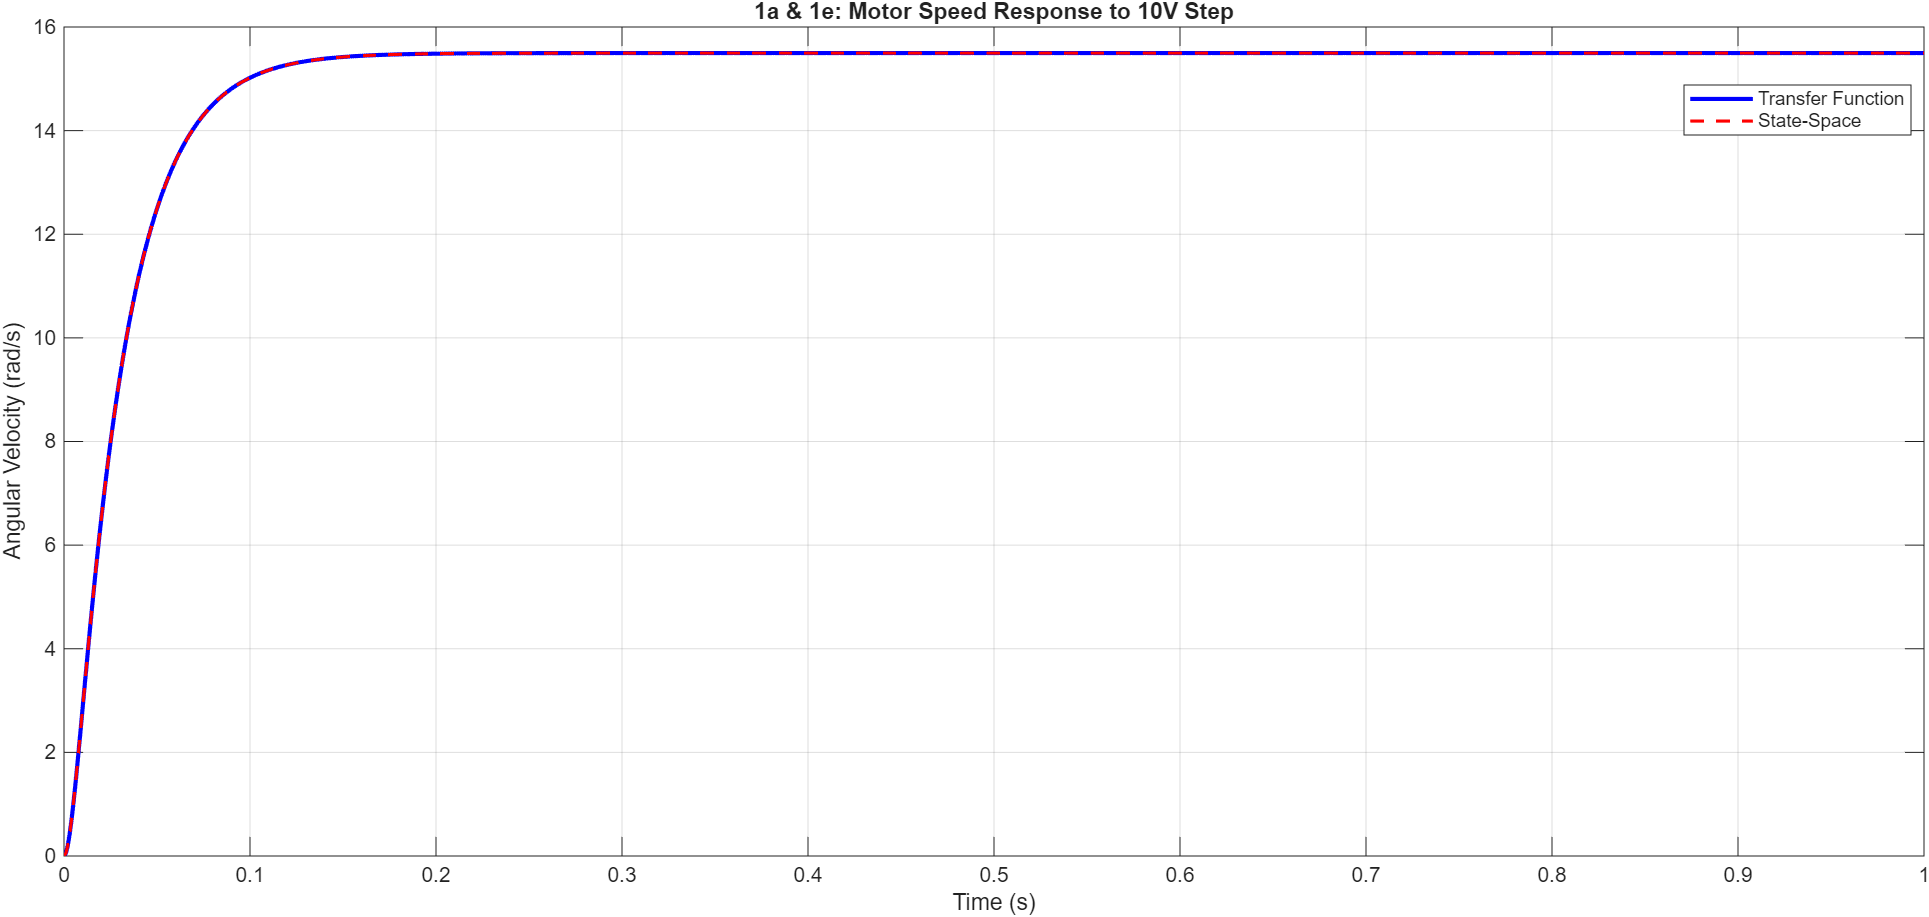
\includegraphics[width=1\textwidth]{1a&e.png}
\end{center}
\textbf{(f)}
\begin{center}
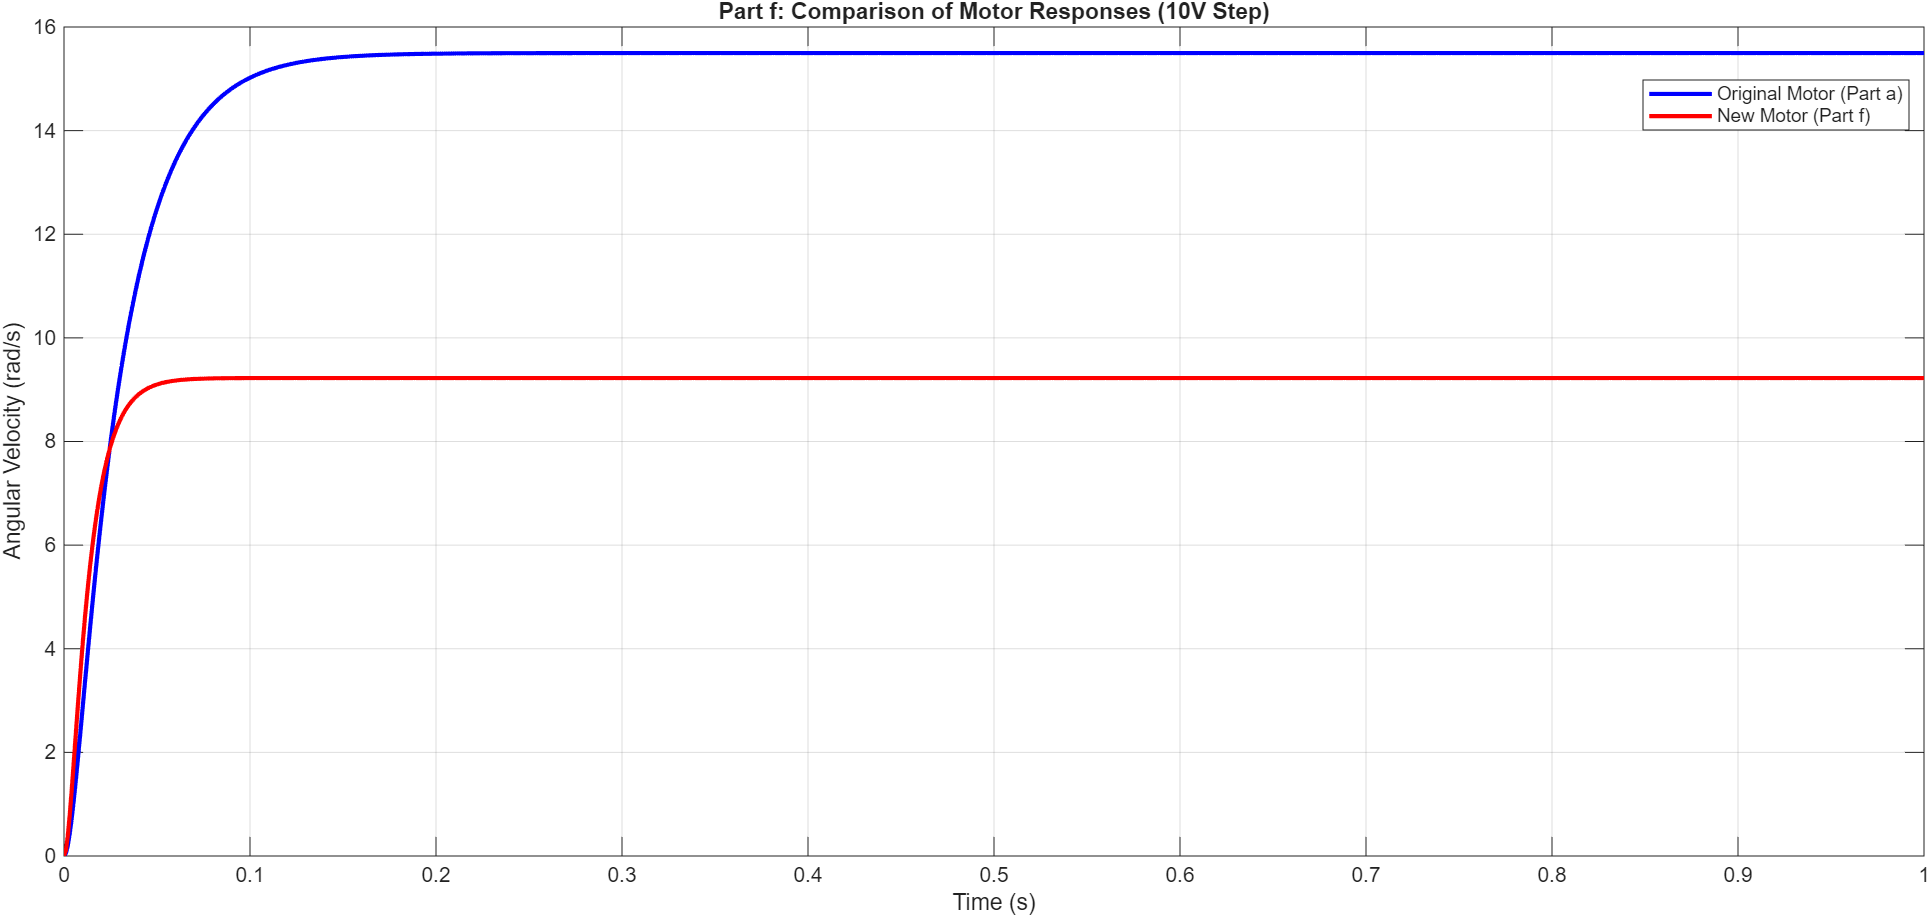
\includegraphics[width=1\textwidth]{1f.png}
\end{center}
\newpage\noindent
\textbf{(g)}
\begin{center}
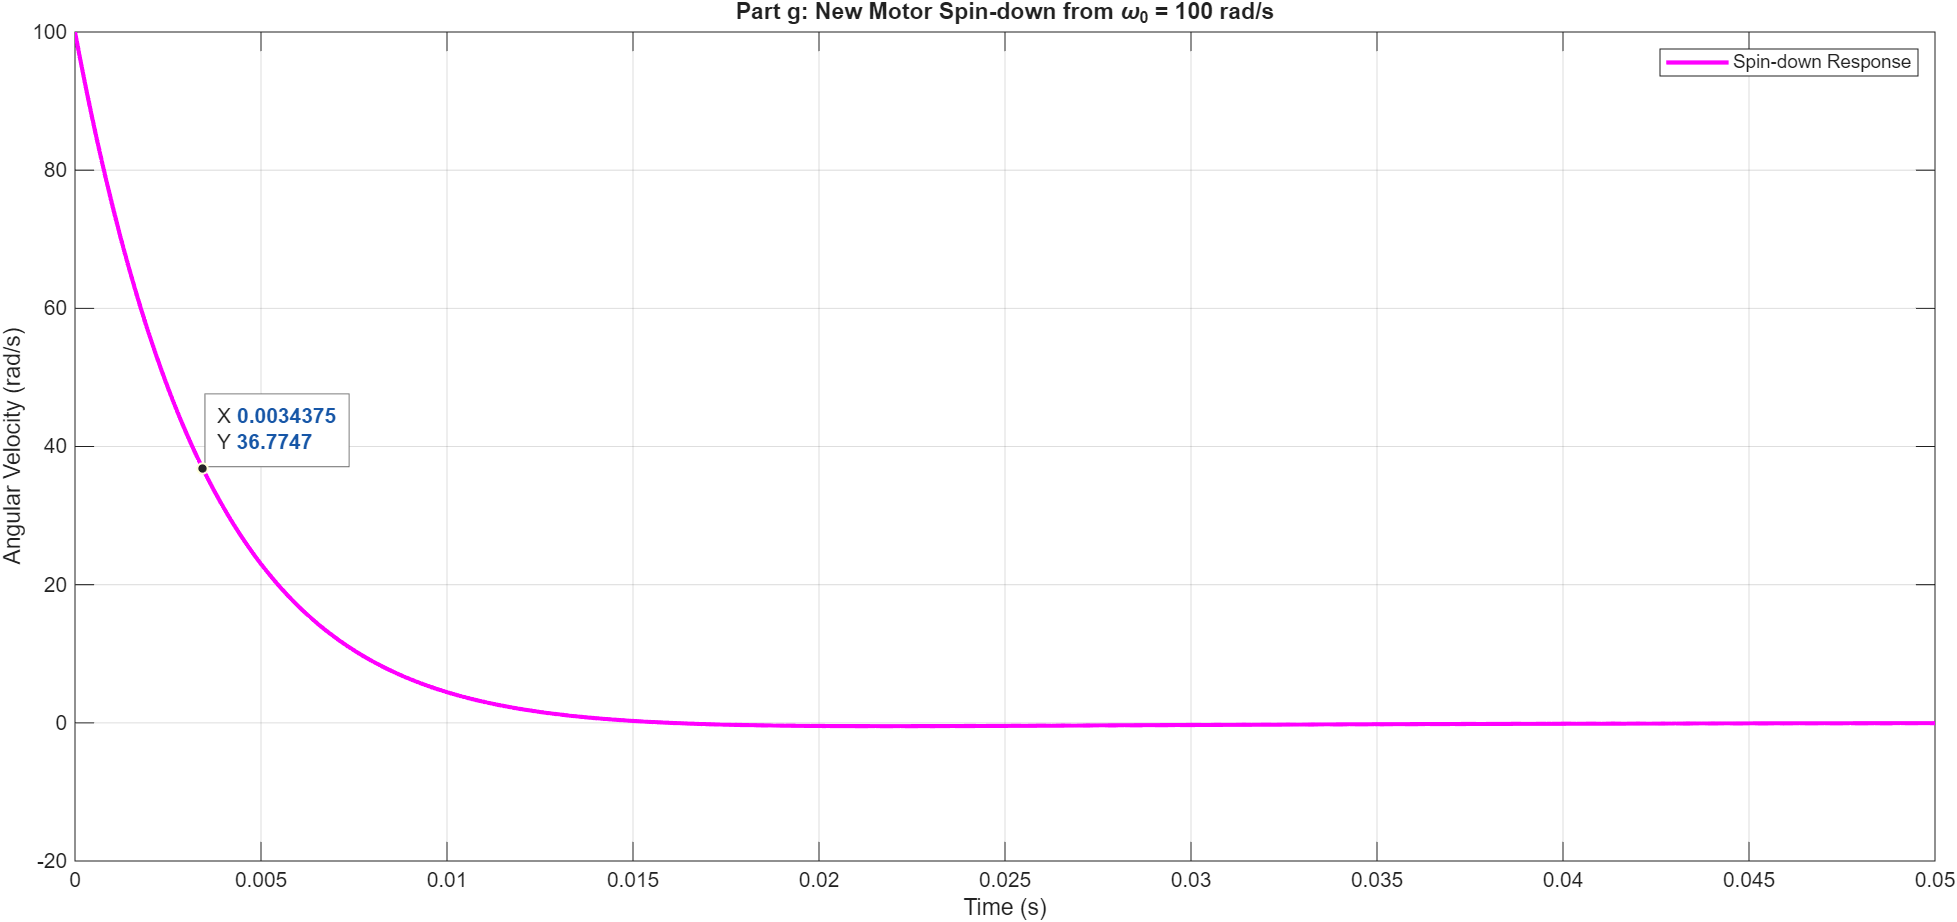
\includegraphics[width=1\textwidth]{1g.png}
\end{center}
\textbf{(k)}
\begin{center}
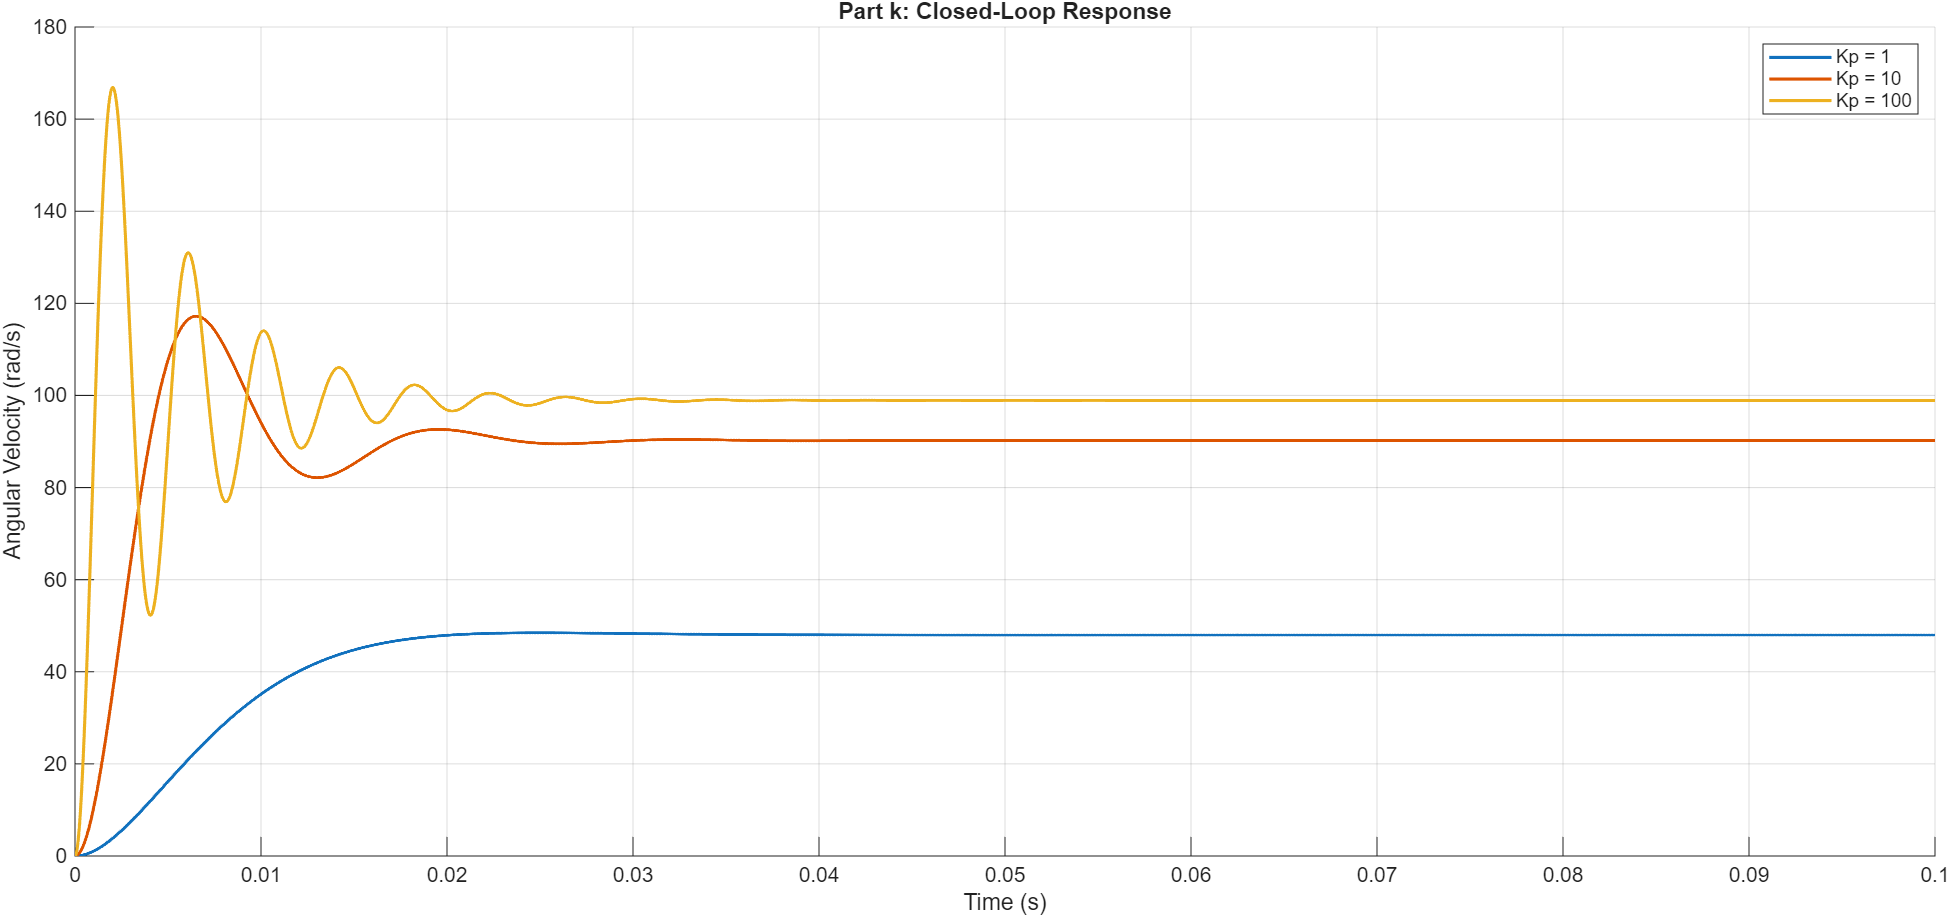
\includegraphics[width=1\textwidth]{1k.png}
\end{center}
\newpage
\section*{2}
\textbf{(a)}
\begin{center}
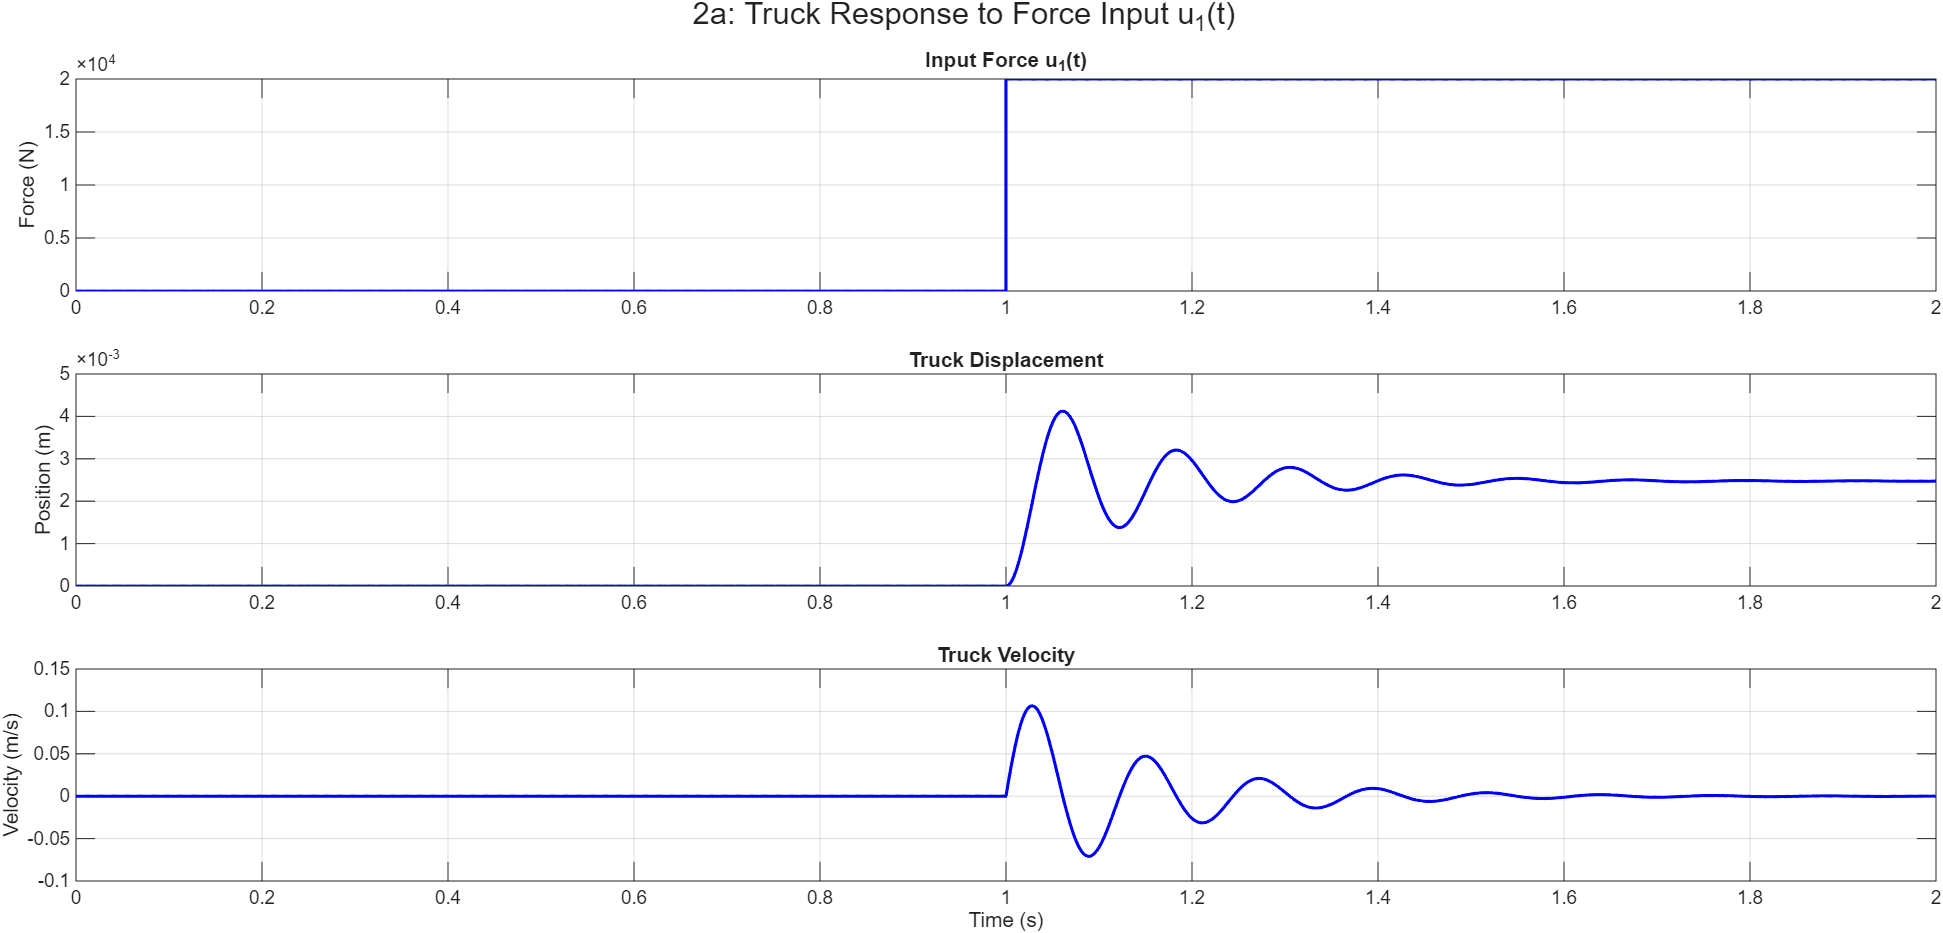
\includegraphics[width=1\textwidth]{2a.png}
\end{center}
\textbf{(c)}
\begin{center}
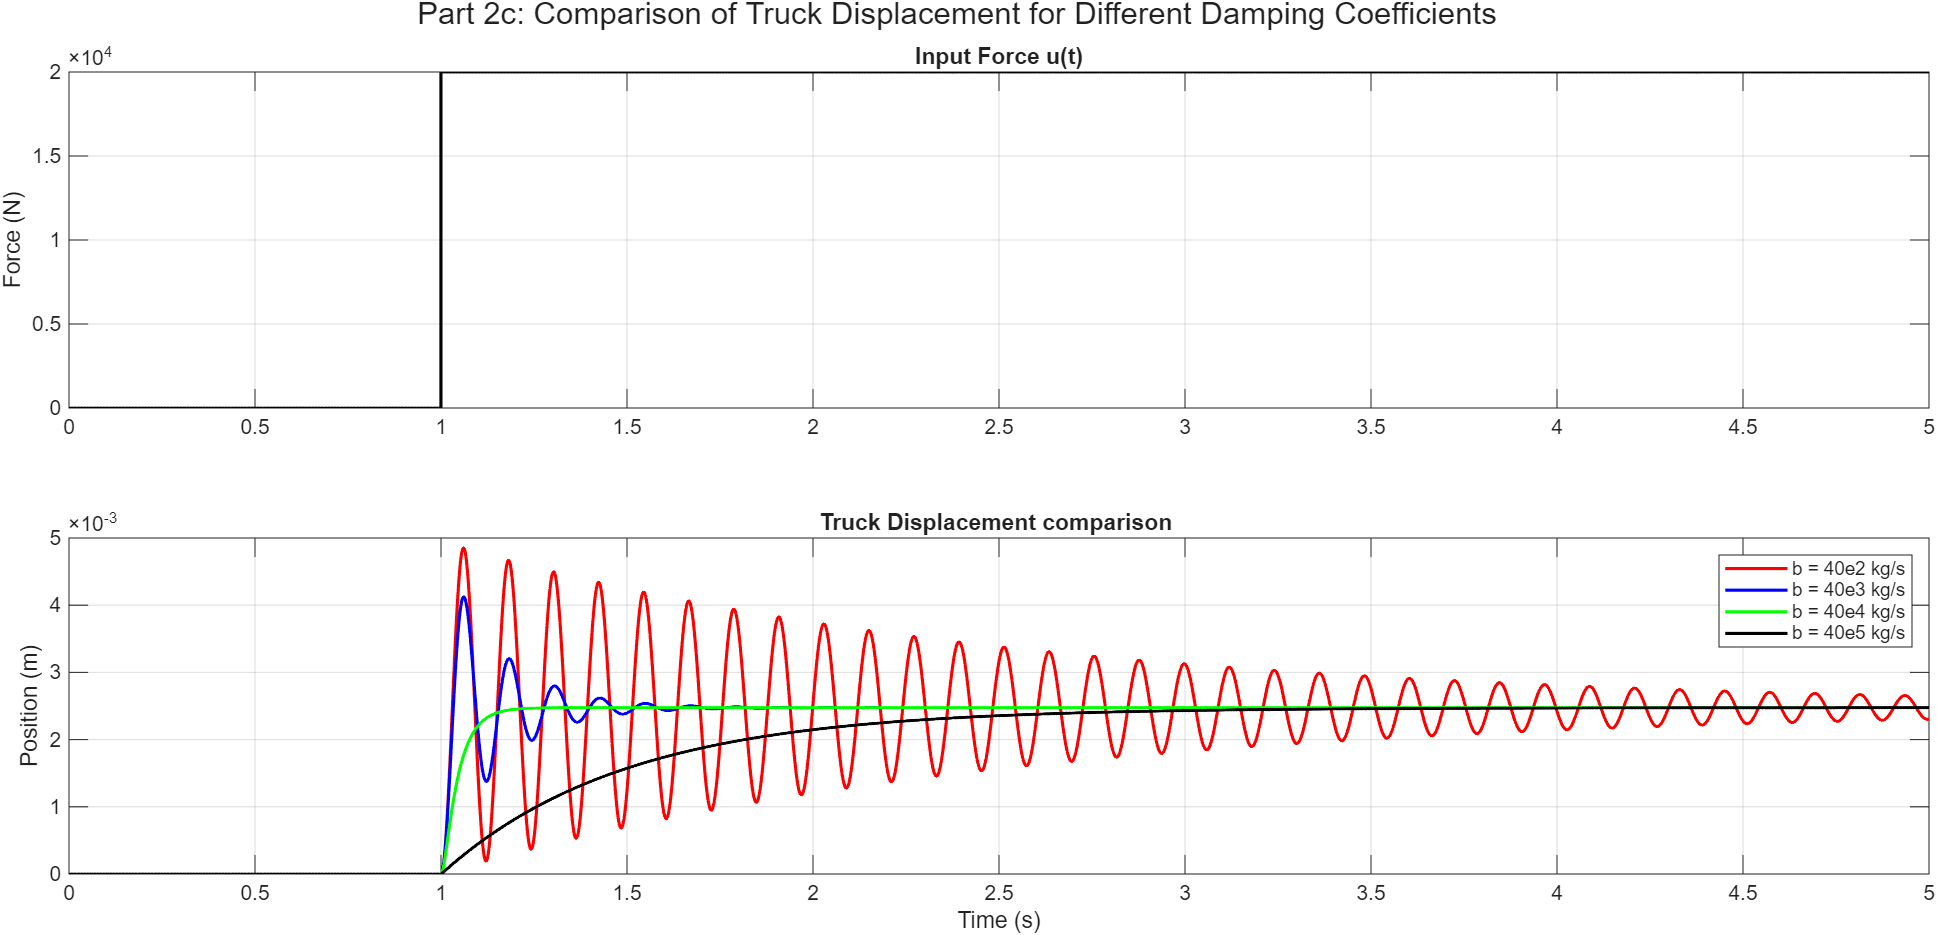
\includegraphics[width=1\textwidth]{2c.png}
\end{center}
\begin{center}
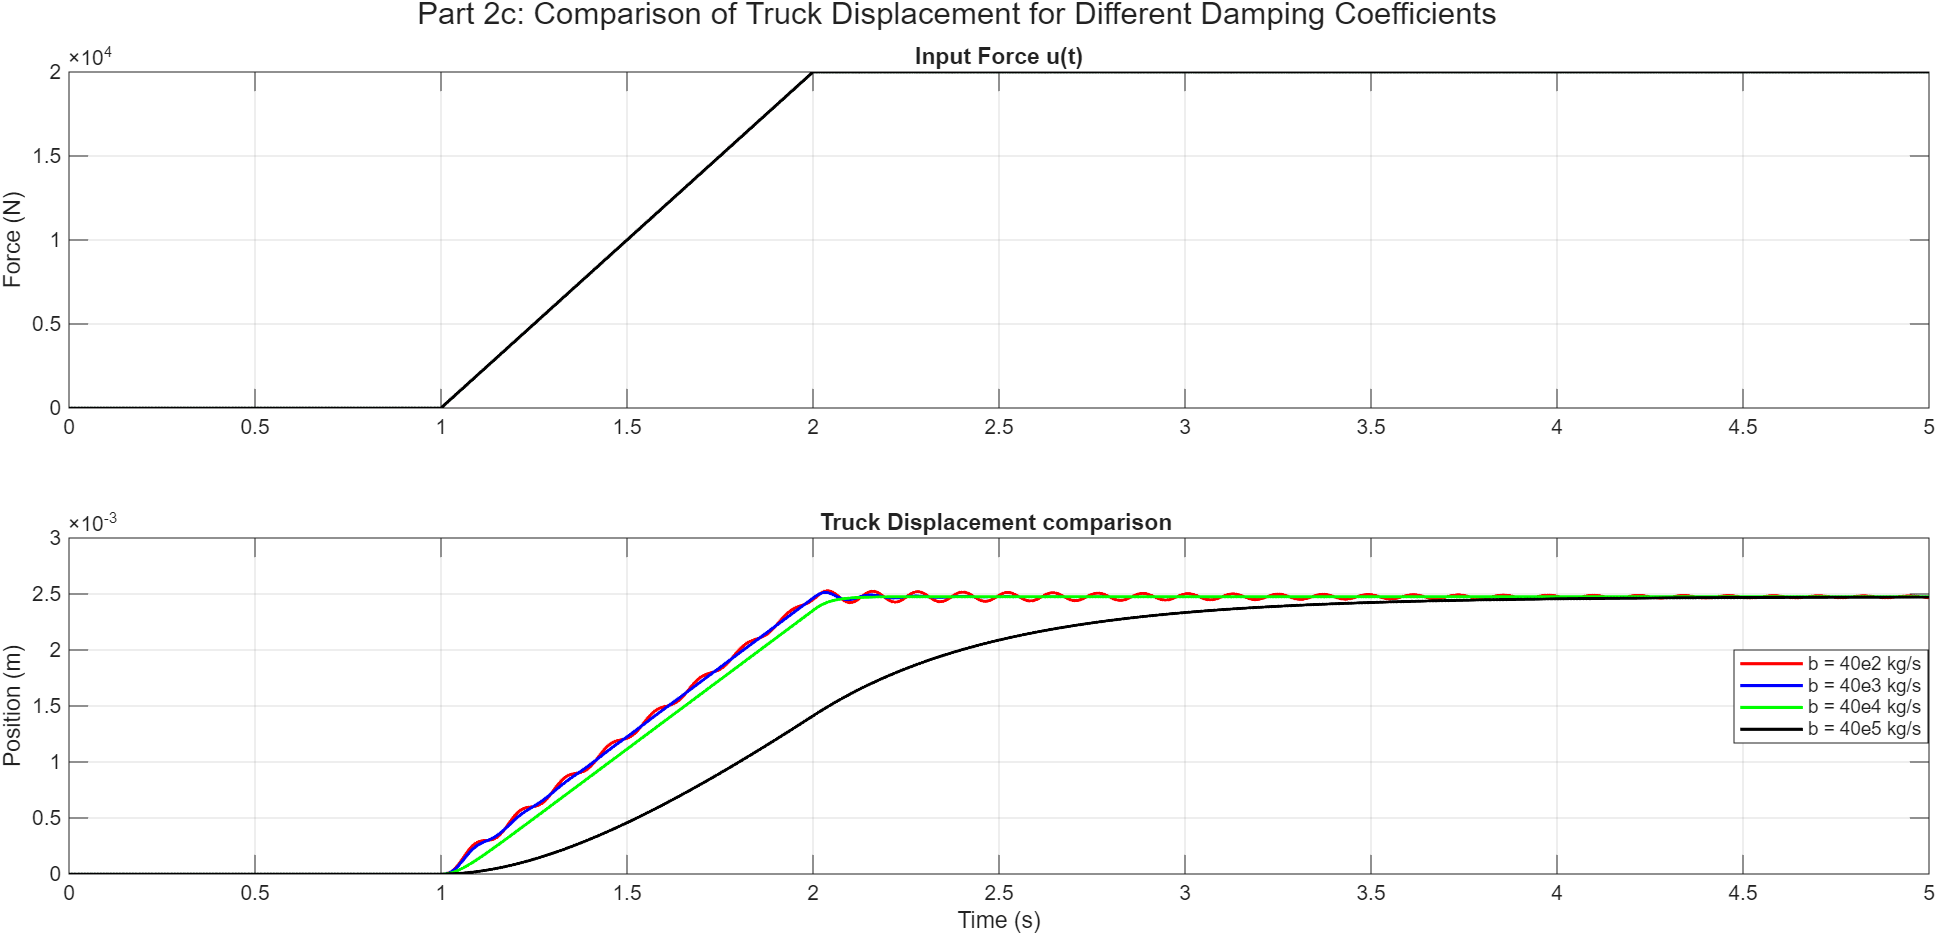
\includegraphics[width=1\textwidth]{2c_1.png}
\end{center}
\textbf{(d)}
\begin{center}
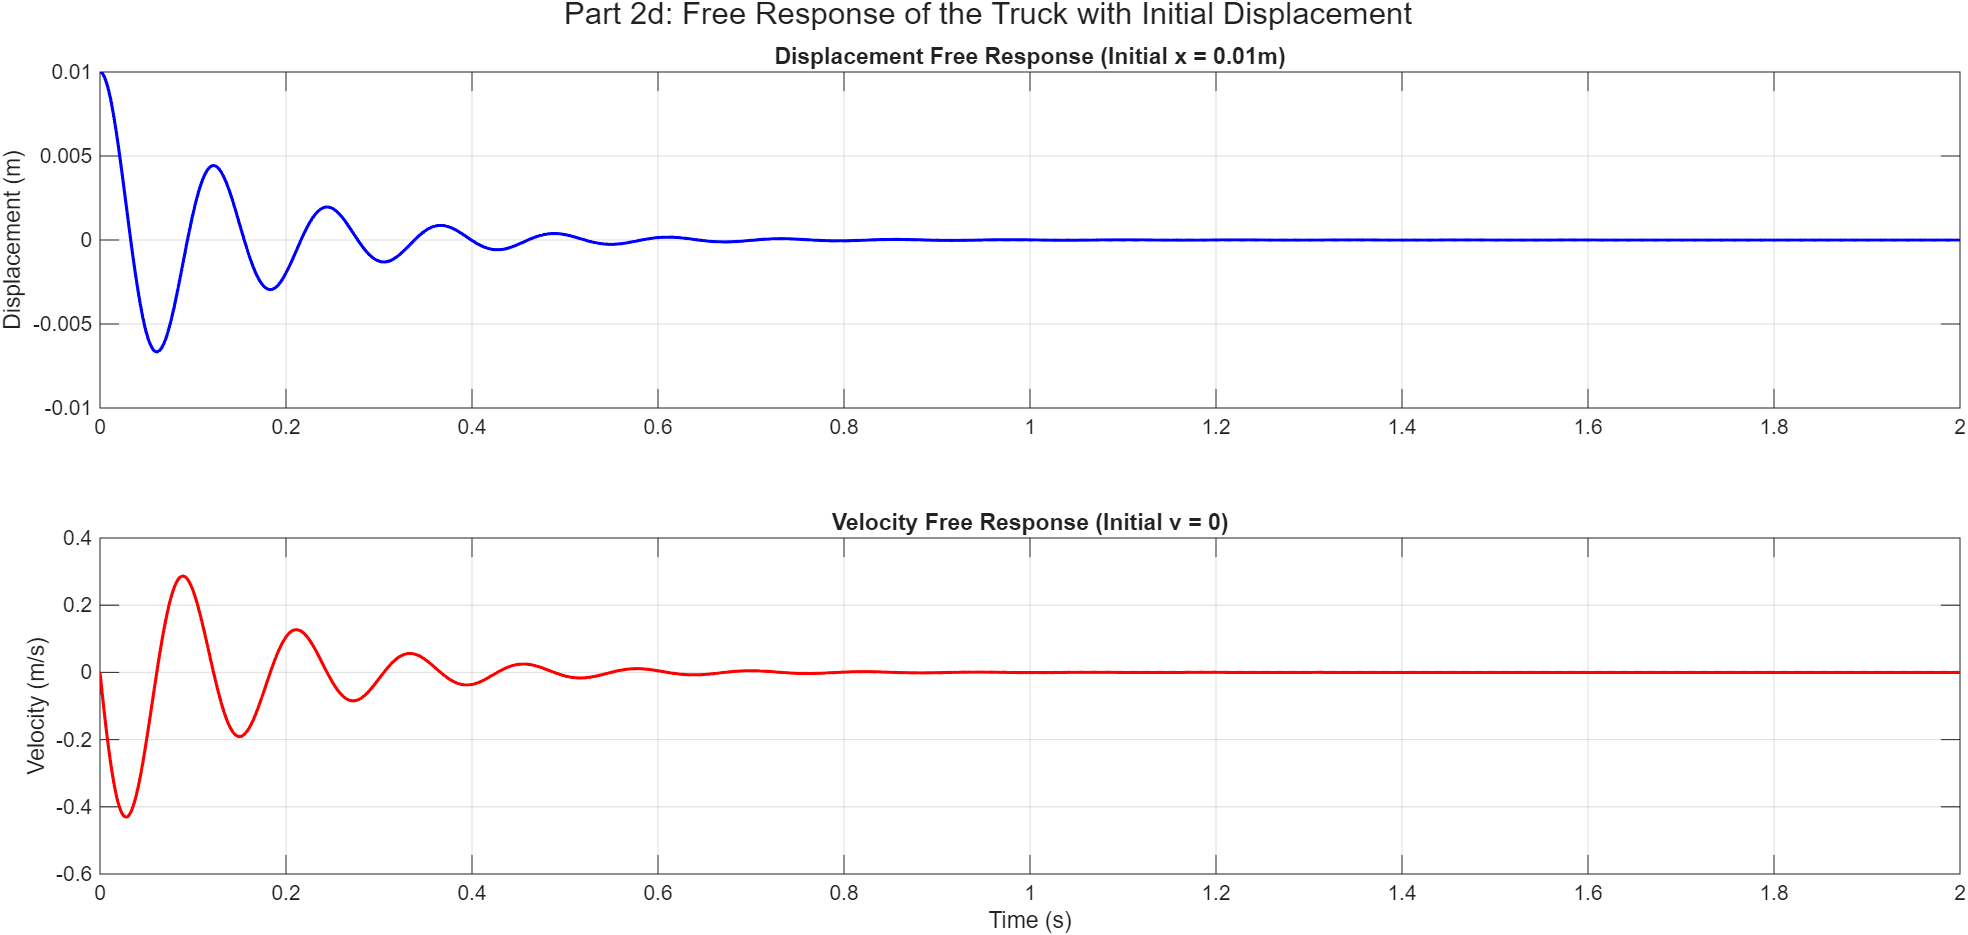
\includegraphics[width=1\textwidth]{2d.png}
\end{center}


\end{document}
